\section{Density Matrices}

%\textcolor{red}{A short summary of the purpose of this section will be helpful. The reviewer/readers would like to establish the chain of logic following your writing. Readers would like to know what information I should anticipate in this section? Can I skip it? Or it is relevant for later understanding? Ideally, here should be a high level description paragraph. Especially, we introduce some unconventional notations. Readers would like to ask: if I really need to use this way of understanding things? Do you have a physical argument that this is the relevant expression to reveal something new?}

%\valert{Here, we discuss the special structures of the density matrix of the Kitaev ground state, such as \textit{strings} and \textit{equivalence classes}. The structures not only reveal the hidden topological nature and features related to the emergent gauge theory, but also imply properties of the entanglement spectrum and entanglement entropy that will be discussed in later sections. }

\valert{
The separability of the entanglement entropy into the gauge part and the matter part~\cite{Yao-Qi} implies a similar pattern in the density matrix. Through the density matrix, we can see the entanglement structure and the emergence of the effective Majorana fermion model in a direct way in the spin representation, instead of relying on the replica approach. In this section, we will see the pattern of the density matrix that implies the separability of the entanglement is encoded in the \textit{equivalence classes} of the \textit{edge configurations} that describe \textit{strings}, both of which are introduced in Section~\ref{sec:density-matrix-whole}. With the basic notion of the strings, we directly derive an analytical form of the density matrix in Section~\ref{sec:density-matrix-calculate}. Using a similar idea, the reduced density matrix is also derived in Section~\ref{sec:density-matrix-reduced}, which will be used as a foundation for the analysis of the entanglement structure. The pattern of the density matrices also directly reflects the identity between the Majorana-fermion representation and the spin representation, which is illustrated in Section~\ref{sec:Emergent-Fermions-at-the-Endpoints}. Such an identity provides a foundation for the microscopic origin of the entanglement structure, especially for the separability of the entanglement into the gauge part and the matter part.
}



\subsection{Edge Configurations, String Operators, and Equivalence Classes}\label{sec:density-matrix-whole}

To make the following discussions more fluent and precise, we denote by $\mathfrak{D}$ the \textit{edge configurations}, which are sets consisting of edges of a honeycomb lattice, and define their \textit{symmetric difference} $\oplus$ as
\[
\mathfrak{D}\oplus\mathfrak{D}' \equiv \mathfrak{D}\cup\mathfrak{D}'-\mathfrak{D}\cap\mathfrak{D}'\]
It can be directly verified to be commutative $\mathfrak{D}\oplus\mathfrak{D}' = \mathfrak{D}'\oplus\mathfrak{D}$ and associative $\lr{\mathfrak{D}_1\oplus\mathfrak{D}_2}\oplus\mathfrak{D}_3 = \mathfrak{D}_1\oplus\lr{\mathfrak{D}_2\oplus\mathfrak{D}_3}$. This algebra has three other properties, (i) $\varnothing\oplus\varnothing = \varnothing$, (ii) $\varnothing\oplus\mathfrak{D}=\mathfrak{D}$, and (iii) $\mathfrak{D}\oplus\mathfrak{D} = \varnothing$, which make it similar to the addition $\mathbb{Z}_2$. An example that illustrates the rule is given below
\[
\wordfig{2.5}{figures/oplus_1}\oplus\wordfig{2.5}{figures/oplus_2} = \wordfig{2.5}{figures/oplus_result},
\]
where thick red edges are those in the edge configurations.

With these, we define \emph{string operators} $\Sigma_\mathfrak{D}$ corresponding to different configurations $\mathfrak{D}$
\begin{equation}\label{equ.string-operator-def}
    \Sigma_\mathfrak{D} \equiv \prod_{\anglelr{ij}\in \mathfrak{D}}\sigma^{\alpha_{ij}}_i\sigma_j^{\alpha_{ij}}
\end{equation}
Because of the anti-commuting feature of the Pauli matrices, we have to notice the order of the product. For example, consider two connected edges. One of them, $\Sigma_{\anglelr{ij}}=\sigma_i^x\sigma_j^x$, is type-$x$, and the other, $\Sigma_{\anglelr{jk}}=\sigma^y_j\sigma^y_k$, is type-$y$. They share a common endpoint $j$. If we want to build $\Sigma_{\anglelr{ij}\oplus\anglelr{jk}}$, we will find that $\lr{\sigma^x_i\sigma_j^x}\lr{\sigma_j^y\sigma_k^y}$ and $\lr{\sigma^x_i\sigma_j^x}\lr{\sigma_j^y\sigma_k^y}$ are different in sign. This example illustrates that the order in which those dimers $\lr{\sigma^{\alpha_{ij}}_i\sigma^{\alpha_{ij}}_j}$ are placed in the product is important in several cases. To make the definition of string operators unique and self-consistent, we have to fix the order. In the subsequent discussion, we assume that all products include ordering information, such that every string operator is uniquely defined. 

A string operator $\Sigma_{\mathfrak{D}}$ is composed of $\mathbb{Z}_2$ dimer operators $\dimer{i}{j}$ within the edge configuration $\mathfrak{D}$. Therefore, multiplying two string operators $\Sigma_{\mathfrak{D}}$ and $\Sigma_{\mathfrak{D}}$ results in a symmetric difference pattern of the two edge configurations $\Sigma_{\mathfrak{D}\oplus\mathfrak{D}'}$. An equivalent statement is that the product of string operators represents the edge configuration algebra $\anglelr{\lrg{\mathfrak{D}},\oplus}$. More precisely, it gives a projective representation with a phase factor $g(\mathfrak{D},\mathfrak{D}')=\pm 1$,
\begin{equation}\label{equ.Sigma-representation}
\Sigma_{\mathfrak{D}}\Sigma_{\mathfrak{D}'} = g(\mathfrak{D},\mathfrak{D}') \Sigma_{\mathfrak{D}\oplus\mathfrak{D}'}.
\end{equation}


Compared to the open strings with endpoints, edge configurations composed of closed loops form a special class, since the expectation values of their corresponding string operators are equal to 1. For example, the simplest closed loop $\de p$ consists of six edges surrounding a plaquette $p$, and the corresponding string operator 
\[
\Sigma_{\de p} = \prod_{\anglelr{ij}\in\de p}\sigma^{\alpha_{ij}}_i\sigma^{\alpha_{ij}}_j = W_p
\]
is a plaquette operator $W_p$ centered at $p$. From the property of $W_p$, string operators of larger loops, as well as edge configurations consisting of multiple loops, can be expressed as combinations of plaquette operators in a specific set $\mathcal{A}$ of plaquettes, in which the loop is exactly the boundary of such a region,
\begin{equation}\label{equ.lattice-Stokes}
    \Sigma_{\de\mathcal{A}} = \prod_{p\in\mathcal{A}}W_p
\end{equation}
as illustrated in \autoref{fig.equivalent}. This is the lattice $\mathbb{Z}_2$ version of the Stokes theorem. As we know, the Kitaev ground state is an eigenvector of plaquette operators with an eigenvalue $+1$. That is, the expectation value of a string operator is equal to one whenever the edge configuration consists of closed loops without open strings. In conclusion, the expectation value of the string operator of the configuration $\mathfrak{D}$ is equal to another configuration $\mathfrak{D}\oplus\de\mathcal{A}$ constructed by adding a loop configuration $\de\mathcal{A}$ to the original one,
\[
\abs{\anglelr{\Sigma_{\de\mathcal{A}}\Sigma_{\mathfrak{D}}}} = \abs{\anglelr{\Sigma_{\mathfrak{D}}}} = \abs{\anglelr{\Sigma_{\de\mathcal{A}\oplus\mathfrak{D}}}}
\]
up to a sign. Such an equation is equivalent to 
\begin{equation}\label{equ.one-loop-equivalence}
\prod_{p\in\mathcal{A}}W_p\anglelr{\Sigma_{\de\mathcal{A}\oplus\mathfrak{D}}}\Sigma_{\de\mathcal{A}\oplus\mathfrak{D}} = \anglelr{\Sigma_{\mathfrak{D}}}\Sigma_{\mathfrak{D}}
\end{equation}
for an arbitrary set $\mathcal{A}$ of plaquettes. Notice that the sign need not be considered since any sign change in the expectation value is exactly canceled by the contribution from the string operator. Although equation \eqref{equ.one-loop-equivalence} shows that two configurations can be related by the loop operator $\Sigma_{\de \mathcal{A}}=\prod_{p\in\mathcal{A}}W_p$, it is not a general formula to relate all kinds of equivalent edge configurations in a unified way. Fortunately, the loop operator $\prod_{p\in\mathcal{A}}W_p$ is composed by $\mathbb{Z}_2$ operators $W_p$, and we also know that the projector $\mathcal{P}^{(p)}$ defined as
\begin{equation}\label{equ.p-projector}
    \mathcal{P}^{(p)}\equiv\prod_{p}\lr{\frac{\mathds{1}+W_p}{2}}
\end{equation}
is invariant after being multiplied by an operator $W_p$
\[
\mathcal{P}^{(p)}W_{p} = \mathcal{P}^{(p)}
\]
This equation can be understood as the plaquette operator $W_{p}$ being absorbed into the projector, and is equivalent to doing nothing. For the same reason, we also have the following relation
\[
\mathcal{P}^{(p)}\prod_{p\in\mathcal{A}}W_p = \mathcal{P}^{(p)}
\]
for arbitrary plaquette configurations $\mathcal{A}$. Combining this relation with \eqref{equ.one-loop-equivalence}, we then have a more general equation to relate the configuration $\mathfrak{D}$ and $\mathfrak{D}\oplus\de\mathcal{A}$,
\begin{equation}\label{equ.string-operator-equivalent}
\mathcal{P}^{(p)}\anglelr{\Sigma_{\de\mathcal{A}\oplus\mathfrak{D}}}\Sigma_{\de\mathcal{A}\oplus\mathfrak{D}} 
= \mathcal{P}^{(p)}\anglelr{\Sigma_{\mathfrak{D}}}\Sigma_{\mathfrak{D}}
\end{equation}

\begin{figure}
    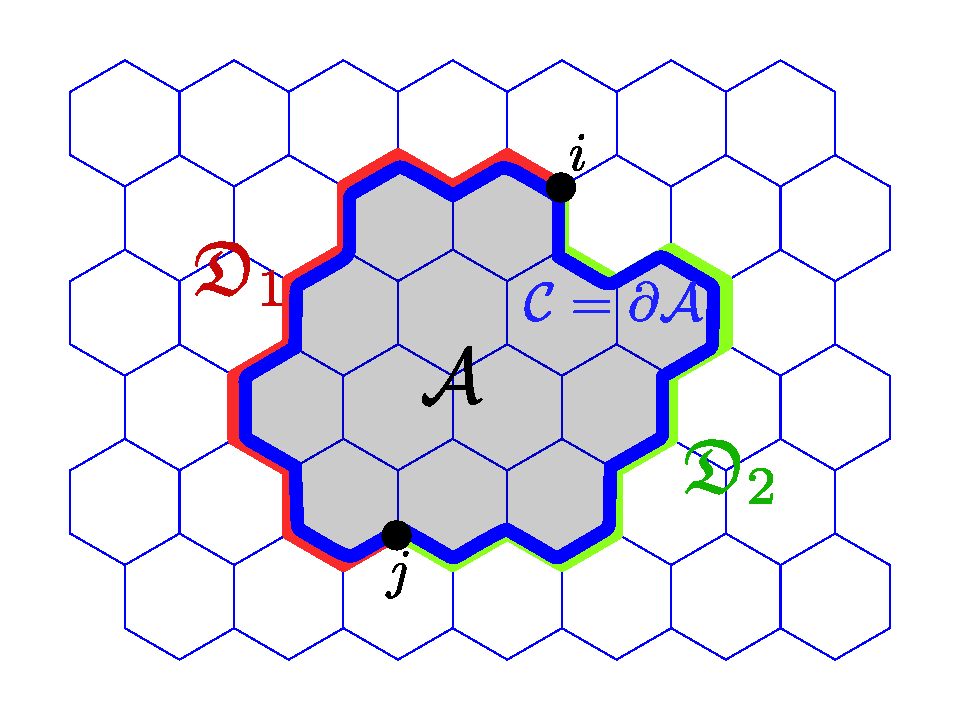
\includegraphics[width=0.45\linewidth]{figures/equivalent_loop.pdf}
    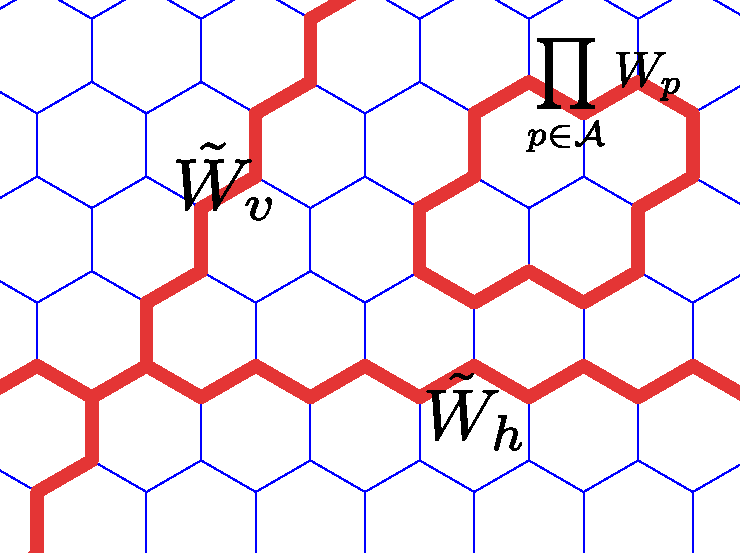
\includegraphics[width=0.45\linewidth]{figures/equivalent.pdf}
    \caption{The left panel shows two equivalent edge configurations $\mathfrak{D}_1\sim\mathfrak{D}_2$ bridged via a loop $\mathcal{C}=\de\mathcal{A}$. The two configurations share the same endpoints $i$ and $j$. The right panel shows three possible ways to get other dimer configurations with the same expectation value of the string operators. The two Wilson loops, $\Tilde{W}_h\equiv \Sigma_{\mathcal{L}_h}$ and $\Tilde{W}_v\equiv \Sigma_{\mathcal{L}_v}$ commute $[\Tilde{W}_h,\Tilde{W}_v]=0$, and neither of them can be constructed by local operators $W_p$'s. Aside from the global Wilson loops, we also have local ones, given by plaquette operators $ W_p$ inside the region $\mathcal{A}$.}
    \label{fig.equivalent}
\end{figure}
Equations~\eqref{equ.one-loop-equivalence} and \eqref{equ.string-operator-equivalent} imply an equivalence relation for edge configurations defined in such a way that two edge configurations $\mathfrak{D}_1$ and $\mathfrak{D}_2$ are \emph{equivalent}, denoted by $\mathfrak{D}_1\sim\mathfrak{D}_2$, if and only if there exists a set $\mathcal{A}$ of plaquettes such that one of the following four conditions holds:
\begin{enumerate}
    \item[(i)] $\mathfrak{D}_1=\mathfrak{D}_2\oplus\de\mathcal{A}$
    \item[(ii)] $\mathfrak{D}_1=\mathfrak{D}_2\oplus\de\mathcal{A}\oplus\mathcal{L}_v$
    \item[(iii)] $\mathfrak{D}_1=\mathfrak{D}_2\oplus\de\mathcal{A}\oplus\mathcal{L}_h$
    \item[(iv)] $\mathfrak{D}_1=\mathfrak{D}_2\oplus\de\mathcal{A}\oplus\mathcal{L}_v\oplus\mathcal{L}_h$
\end{enumerate} 
$\mathcal{L}_v$ and $\mathcal{L}_h$ are the global loop that circles the torus in the vertical and horizontal directions, the corresponding string operators of which are $\Tilde{W}_v\equiv\Sigma_{\mathcal{L}_v}$ and $\Tilde{W}_h\equiv\Sigma_{\mathcal{L}_h}$, respectively, as illustrated in the right panel of \autoref{fig.equivalent}. Equivalent configurations are collected into \emph{equivalence classes} $[\mathfrak{D}^c]=\lrg{\mathfrak{D}:\mathfrak{D}\sim\mathfrak{D}^c}$ characterized by each character $\mathfrak{D}^c$. The right panel of Fig.~\ref{fig.equivalent} shows that the two equivalent edge configurations must share the same set of endpoints, giving a simple way to identify equivalent edge configurations. In other words, there is a one-to-one correspondence between an equivalence class for edge configurations $[\mathfrak{D}]$ and the \textit{set of endpoints} of the character configuration $\mathfrak{D}$, denoted by $\mrm{EP}\lr{\mathfrak{D}}$. 
\begin{figure}
    \centering
    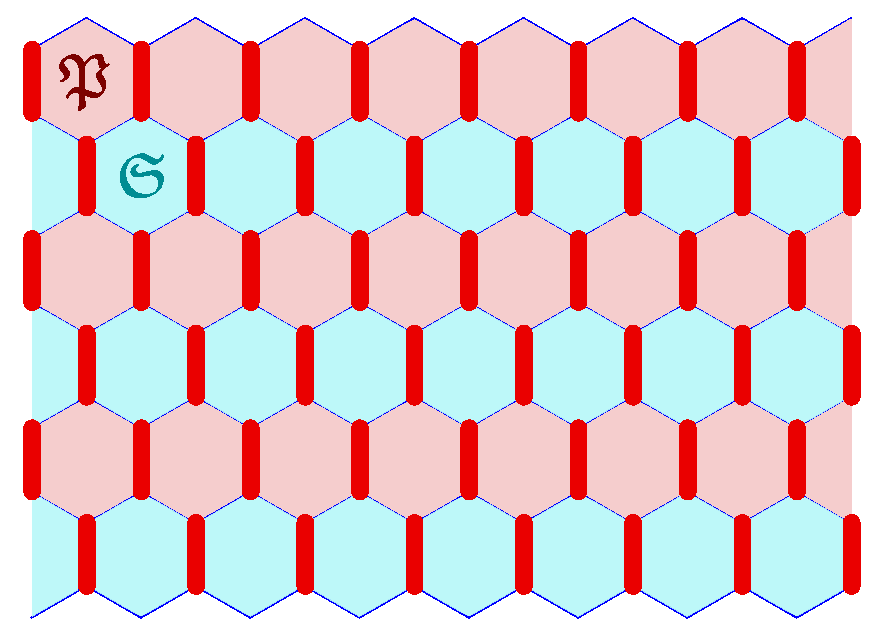
\includegraphics[width=0.48\linewidth]{figures/S-P-dimer-gas.pdf}
    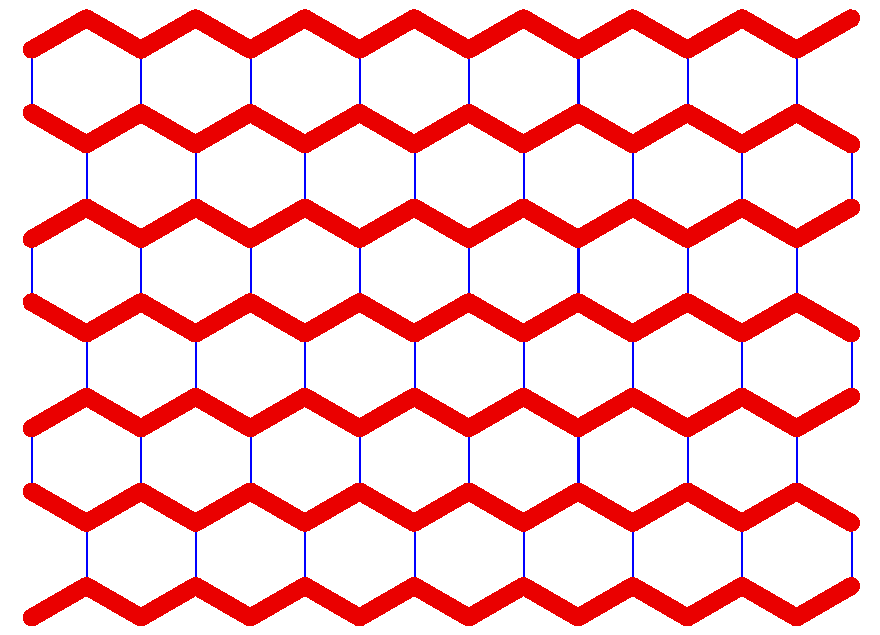
\includegraphics[width=0.48\linewidth]{figures/snake-and-dimer-gas.pdf}
    \caption{The left panel illustrates the plaqeutte configurations $\mathfrak{P}$ and $\mathfrak{S}$ as well as the edge configuration $\mathfrak{D}_Z$. The set of plaquettes in pink is denoted by $\mathfrak{P}$, while the set containing those in pink-blue is denoted by $\mathfrak{S}$. The edge configuration $\mathfrak{D}_Z$ consists of all of the red $z$-directional edges in the system, as shown in the above figure. The right panel illustrates the zigzag configuration $\mathfrak{D}_{zz}$ consisting of edges at all the horizontal loops. Such an edge configuration is also the boundary of both $\mathfrak{P}$ and $\mathfrak{S}$, for which we can write $\mathfrak{D}_{zz} = \de\mathfrak{P} = \de\mathfrak{S}$. Note that $\Sigma_{\mathfrak{D}_Z}=\Sigma_{\mathfrak{D}_{zz}}$ although $\mrm{EP}(\mathfrak{D}_Z)\neq \mrm{EP}(\mathfrak{D}_{zz})=\varnothing$} 
    \label{fig.S-P-dimer-gas}
\end{figure}

String operators of edge configurations in the same class have the same magnitude of expectation values,
\[
\abs{\anglelr{\Sigma_{\mathfrak{D}}}} = \abs{\anglelr{\Sigma_{\mathfrak{D}'}}} \quad\text{if $\mathfrak{D}\sim\mathfrak{D}'$}
\]
hence contribute the same weight to the density matrix. Nevertheless, it is still possible for two configurations from different classes to have the same weight contribution to the density matrix. There are a type of plaquette configurations, $\mathfrak{P}$ and $\mathfrak{S}$, that transform an edge configuration $\mathfrak{D}$ to $\mathfrak{D}\oplus\mathfrak{D}_Z$ because of the following relation
\begin{equation}\label{equ.P-S-dimer}
    \prod_{p\in\mathfrak{P}}W_p = \prod_{p\in\mathfrak{S}}W_p = \prod_{\anglelr{ij}\in \mathfrak{D}_Z}\sigma_i^z\sigma_{j}^z = \Sigma_{\mathfrak{D}_Z}.
\end{equation}
The plaquette configurations $\mathfrak{P}$ and $\mathfrak{S}$ as well as the edge configuration $\mathfrak{D}_Z$ are illustrated in the left panel of \autoref{fig.S-P-dimer-gas}. The edge configuration $\mathfrak{D}_Z$ is composed of the $z$-directional dimers all over the system. The plaquette configuration $\mathfrak{P}$ contains all the plaquettes at the even horizontal layers, while $\mathfrak{S}$ is the complement of $\mathfrak{P}$. The endpoint configuration $\mrm{EP}(\mathfrak{D}_Z)$ is simply the set of all the lattice sites in the system. On the other hand, the operators $\prod_{p\in\mathfrak{P}}W_p$ and $\prod_{p\in \mathfrak{S}}W_p$ is also equal to the string operator of the zigzag edge configuration $\mathfrak{D}_{zz}$, a set of all the $x$- and $y$-edges, as illustrated in the right panel of \autoref{fig.S-P-dimer-gas}
\begin{equation}\label{equ.M-MZ-complement}
\prod_{p\in\mathfrak{P}}W_p = \prod_{p\in\mathfrak{S}}W_p  = \Sigma_{\mathfrak{D}_{zz}}
\end{equation}
because $\de\mathfrak{P} = \de\mathfrak{S} = \mathfrak{D}_{zz}$.  Unlike $\mathfrak{D}_Z$, this edge configuration has no endpoints, $\mrm{EP}(\mathfrak{D}_{zz})=\varnothing$, and is equivalent to vacuum. So, we need to keep in mind that every two configurations, $\mathfrak{D}\oplus\mathfrak{D}_Z$ and $\mathfrak{D}\oplus\mathfrak{D}_{zz}$, give an identical string operator, although they are not equivalent.

We would also like to show that the physical meaning of the operator $\Sigma_{\mathfrak{D}_Z}$ is exactly the total fermion parity of the $c$-Majorana fermions. Because the expectation values of fluxes are fixed to be $\anglelr{W_p}=+1$ in the ground state, we directly know that the expectation value of $\Sigma_{\mathfrak{D}_Z}$ is equal to $+1$ directly from equation \eqref{equ.P-S-dimer} 
\begin{equation}\label{equ.fermion-parity-dimer-rep}
    \anglelr{\Sigma_{\mathfrak{D}_Z}}=1
\end{equation}
It is also worth mentioning that the combination of the plaquette operator over $\mathfrak{P}$ and the string operators containing $z$-dimers all over the lattice is equal to multiplying all edges in the entire lattice $\Lambda$ together
\begin{equation}\label{equ.fermion-parity-spin-rep}
    \lr{\prod_{p\in\mathfrak{P}}W_p} \Sigma_{\mathfrak{D}_Z} = \prod_{\anglelr{ij}\in\Lambda}\dimer{i}{j} = \mathds{1}
\end{equation}
This is nothing but the identity operator of the entire system because of the geometry of the honeycomb lattice. We can understand equations \eqref{equ.fermion-parity-dimer-rep} and \eqref{equ.fermion-parity-spin-rep} in the sense of fermion parity. In our convention, the gauge is fixed as $u_{ij}=1\forall\anglelr{ij}$, therefore, the string operator corresponding to the edge configuration that contains all of the edges in the lattice, as appeared in the last equation, transforms into the fermion parity operator $\hat{\bog{\pi}}$ up to a phase~\footnote{Two distinct Majorana fermions, say $c_1$ and $c_2$, can combine to form a normal fermion degree of freedom $f$ in a way that $f=\frac{1}{2}\lr{c_1+ic_2}$ and $f^\dagger=\frac{1}{2}\lr{c_1-ic_2}$. In this way, the fermion parity operator represented using the Majorana fermions becomes $\hat{\bog{\pi}}\equiv(-1)^{f^\dagger f}=ic_1c_2$. In a more general sense, the fermion parity operator is equal to the multiplication of all the Majorana fermions $\prod_i c_i$ up to a phase.}
\begin{equation}\label{equ.total-fermion-parity-entire-system}
    \prod_{\anglelr{ij}\in\Lambda}\dimer{i}{j}\to \prod_{\anglelr{ij}\in \Lambda}ic_ic_j
\propto \prod_{i\in\Lambda}c_i\propto \hat{\bog{\pi}}
\end{equation}
This is also due to the geometric feature of the honeycomb lattice, in which three connected edges share a lattice site. Similarly, the operator $\Sigma_{\mathfrak{D}_Z}$ in the Majorana representation is also equal to the fermion parity operator
\begin{equation}\label{equ.total-fermion-parity-Sigma-Z}
    \Sigma_{\mathfrak{D}_Z} \to \prod_{\anglelr{ij}\in\mathfrak{D}_Z}ic_ic_j\propto \prod_{i\in\Lambda}c_i\propto\hat{\bog{\pi}},
\end{equation}
because, as we will emphasize later, Majorana fermions emerge at the endpoints of each $z$-directional dimer, thus $\mrm{EP}(\mathfrak{D}_Z)$ is exactly the whole lattice system $\Lambda$. From the Majorana fermion point of view, the fermionic representation of the Kitaev Hamiltonian \eqref{equ.MF-Hamiltonian} is quadratic. As a consequence, the total fermion parity of the whole system should be conserved and must be $+1$ on a torus~\cite{Fu-Knolle-Perkins-2018}. This fermion parity degree of freedom is emergent only in the Majorana representation, and should be fixed by the intrinsic property of the spin operators in the physical spin representation. This is why the expectation value of the operator $\Sigma_{\mathfrak{D}_Z}$ is $+1$. 

Aside from the convenience arising from the fact that endpoint-point sets uniquely determine the equivalent class, the physical picture about the equivalence classes and endpoint sets also implies that a Pauli string in the spin representation is identical to the two Majorana fermions residing on the endpoints of the string. This can be seen in the \textit{commutation} among the endpoints of strings~\cite{Kitaev, fermion-and-string}. More details will be discussed in Section \ref{sec:Emergent-Fermions-at-the-Endpoints}. 


\subsection{Density Matrix of the Kitaev Ground State on a Torus}\label{sec:density-matrix-calculate}

So far, we have known two crucial points for constructing the density matrix. The first one is that finite spin-correlation functions of the Kitaev ground state must be of the following form
\[
\anglelr{\prod_{\anglelr{ij}\in \mathfrak{D}}\sigma^{\alpha_{ij}}_i\sigma^{\alpha_{ij}}_j} = \anglelr{\Sigma_{\mathfrak{D}}} \equiv \mathfrak{C}_{\mathfrak{D}}
\]
Otherwise, the correlation function vanishes. From now on, we denote by $\mathfrak{C}_{\mathfrak{D}}$ the expectation values of the string operator corresponding to the edge configuration $\mathfrak{D}$. The other is that every edge configuration in the same equivalence class gives the same weight to the density matrix, so we can sort terms in the expansion \eqref{equ.rho-starting} into equivalence classes
\begin{equation}\label{equ.class-sum}
    \sum_{\mathfrak{D}}\mathfrak{C}_{\mathfrak{D}}\Sigma_\mathfrak{D} = \sum_{[\mathfrak{D}^c]}\sum_{\mathfrak{D}\in[\mathfrak{D}^c]}\mathfrak{C}_{\mathfrak{D}}\Sigma_\mathfrak{D}
\end{equation}
From \eqref{equ.string-operator-equivalent}, we also know that every term of \eqref{equ.class-sum} in an equivalence class can be related to each other via the projector $\mathcal{P}^{(p)}$. Altogether, applying a projector $\mathcal{P}^{(p)}$ is exactly factorizing the density matrix into groups that include every edge configuration in an equivalence class $\sum_{\mathfrak{D}\in [\mathfrak{D}^c]}$, and the form of the density matrix should contain only characters of different classes $[\mathfrak{D}^c]$. Therefore, we anticipate that the form of the density matrix is of the following form
\begin{equation}\label{equ.rho-factorization}
    \rho = C \mathcal{P}_{\mrm{topo}} \sum_{[\mathfrak{D}]} \mathcal{P}^{(p)} \mathfrak{C}_{\mathfrak{D}} \Sigma_{\mathfrak{D}}
\end{equation}
where the topological Wilson-loop projector 
\[
\mathcal{P}_{\mrm{topo}}\equiv \lr{\frac{\mathds{1}+\Tilde{W}_h}{2}}\lr{\frac{\mathds{1}+\Tilde{W}_v}{2}}
\]
is imposed to include configurations related by global loops $\mathcal{L}_v$ and $\mathcal{L}_h$ illustrated in \autoref{fig.equivalent}. The constant $C$ is the normalization factor, which will be determined by imposing the constraint $\Tr\rho = 1$. Carrying out the trace 

\begin{align}\label{equ.rho-direct-trace-1}
    \Tr\rho &= \frac{C}{4} \sum_{[\mathfrak{D}]} \mathfrak{C}_{\mathfrak{D}} \Tr\lr{\mathcal{P}^{(p)}\Sigma_{\mathfrak{D}}} \nonumber\\
    &= \frac{C}{2^{2+N_p}} \sum_{[\mathfrak{D}]} \sum_{\mathcal{A}}'\Tr\lrm{ \lr{2\prod_{p\in\mathcal{A}} W_p}\Sigma_{\mathfrak{D}}}
\end{align}
The coefficient $1/4$ in the first line originates from the denominator of $\mathcal{P}_{\mrm{topo}}$. The two global Wilson-loop operators drop out because neither the local plaquette operators nor the string operators can annihilate them to yield the identity; consequently, their contributions vanish upon taking the trace. The summation of plaquette operators arises from the expansion of $\mathcal{P}^{(p)}$
\begin{align}\label{equ.W-prod-expansion}
    \prod_{p}\lr{\mathds{1}+W_p} &= \lr{\mathds{1}+\prod_{p}W_p}\sum'_{\mathcal{A}}\prod_{p\in\mathcal{A}}W_p \nonumber\\
    &= 2\sum'_{\mathcal{A}}\prod_{p\in\mathcal{A}}W_p.
\end{align}
with $\mathcal{A}$ denoting different sets of plaqette configurations defined in \eqref{equ.lattice-Stokes}. We point out that, due to the identity $\prod_{p}W_p=\mathds{1}$, the loop constructed by $\prod_{p\in \mathcal{A}}W_p$ is identical to that constructed by $\prod_{p\in \overline{\mathcal{A}}}W_p$ with $\overline{\mathcal{A}}$ representing the complement of $\mathcal{A}$. Therefore, we only need to sum over distinct loops, and the sum with a prime symbol on top in \eqref{equ.W-prod-expansion} precisely stands for such a summation. The only two terms that contribute to the trace in \eqref{equ.rho-direct-trace-1} are (i) $\mathcal{A}=\varnothing$ and $\mathfrak{D}\sim \varnothing$ and (ii) $\mathcal{A}=\mathfrak{P}$ and $\mathfrak{D}\sim\mathfrak{D}_Z$. Therefore, \eqref{equ.rho-direct-trace-1} is equal to 
\[
\Tr\rho = \frac{C}{2^{N_p}}\Tr\mathds{1} = \frac{C}{2^{-N+N_p}}
\]
To make the trace equal to $1$, we require $C = 2^{-N+N_p}$. In the end, we obtain the exact form of the density matrix
\begin{equation}\label{equ.density-matrix}
    \rho =  \frac{1}{2^{N-N_p}}\mathcal{P}_{\mrm{topo}}\mathcal{P}^{(p)}\sum_{[\mathfrak{D}]}\mathfrak{C}_{\mathfrak{D}}\Sigma_{\mathfrak{D}}
\end{equation}
Because $[W_p,\Sigma_\mathfrak{D}]=0\;\forall p,\mathfrak{D}$, the projectors $\mathcal{P}^{(p)}$ and $\mathcal{P}_{\mrm{topo}}$ commute with the summation part consisting of string operators. This is also a manifestation of the separability of the $c$-Majorana fermion sector from the gauge sector, which will be elucidated in later sections.


\subsection{Reduced Density Matrix}\label{sec:density-matrix-reduced}

\valert{
Information about the many-body entanglement of a state is encoded in the reduced density matrix $\rho_A$, knowing which is the first step in investigating the entanglement structure. Here, we introduce an intuitive approach to obtain the reduced density matrix, where the identity between the spin representation and the Majorana-fermion representation is demonstrated again, similar to the previous section. Nevertheless, we also provide a rigorous derivation of how to carry out the trace directly in Appendix~\ref{appendix:reduced-density0matrix}. 
}

The property of a reduced density matrix is pretty much the same as the density matrix of the entire system, since both are designed to give the expectation values of observables in the way that $\anglelr{\mathcal{O}_A}=\Tr\lr{\rho\mathcal{O}_A}=\Tr_A\lr{\rho_A\mathcal{O}_A}$, for any observable $\mathcal{O}_A$ with support $A$. In the Kitaev model, observables possessing finite expectation values are string operators. Therefore, the reduced density matrix can be expressed in terms of string operators $\Sigma_\mathfrak{D}$, with $\mathfrak{D}$ entirely inside $A$, accompanied by their expectation values $\mathfrak{C}_\mathfrak{D}$,
\begin{equation}\label{equ.rho-A-raw-guess}
    \rho_A \propto\sum_{\mathfrak{D}\subset A}\mathfrak{C}_\mathfrak{D} \Sigma_\mathfrak{D}
\end{equation}
The equivalent configurations can be sorted in the same way as in the previous section, then the summation can be rewritten as a summing of equivalent classes with the projector $\mathcal{P}^{(p)}_A$ of dimension $2^{N^A-N^A_p}$, which only includes plaquettes inside $A$,
\begin{equation}\label{equ.p-proj-A}
    \mathcal{P}^{(p)}_A = \prod_{p\in A}\lr{\frac{\mathds{1}+W_p}{2}}
\end{equation}
The final form of the reduced density matrix is then
\[
\rho_A = C\mathcal{P}^{(p)}_A\sum_{[\mathfrak{D}]\subset A}\mathfrak{C}_{\mathfrak{D}}\Sigma_{\mathfrak{D}}
\]
The condition $[\mathfrak{D}]\subset A$ below the summation means choosing equivalence classes such that each class contains at least one configuration that is entirely contained within $A$. Recall the correspondence between endpoint sets and equivalent classes, the condition is also equivalent to choosing classes $[\mathfrak{D}]$ such that $\mrm{EP}(\mathfrak{D})\subset A$. The constant $C$ is a normalization coefficient to be determined by imposing the normalization condition $\Tr_A\rho_A=1$,
\begin{align*}
    \Tr_A\rho_A &= C\sum_{[\mathfrak{D}]\subset A} \mathfrak{C}_\mathfrak{D} \Tr_A\lrm{\mathcal{P}^{(p)}_A \Sigma_\mathfrak{D}} \\
    &= \frac{C}{2^{N^A_p}}\sum_{\mathcal{A}_p}\sum_{[\mathfrak{D}]\subset A} \mathfrak{C}_\mathfrak{D} \Tr_A\lrm{ \lr{\prod_{p\in\mathcal{A}_p}W_p} \Sigma_\mathfrak{D}} \\
    &= \frac{C}{2^{N^A_p}}\Tr_A\mathds{1}_A = C2^{N^A - N^A_p} = 1
\end{align*}
Therefore, the final form of the reduced density matrix is as follows.
\begin{equation}\label{equ.red-den-mat-sim-con}
    \rho_A = \frac{1}{2^{N^A-N^A_p}} \mathcal{P}^{(p)}_A\sum_{[\mathfrak{D}]\subset A}\mathfrak{C}_{\mathfrak{D}}\Sigma_{\mathfrak{D}}
\end{equation}
The form \eqref{equ.red-den-mat-sim-con} is the same as the density matrix \eqref{equ.density-matrix} as we anticipated. 


\subsection{Emergent Fermions at the Endpoints of Strings -- Equivalence between Spin and Fermion Representation}\label{sec:Emergent-Fermions-at-the-Endpoints}

%\textcolor{red}{The first paragraph should be high level explaination first then detail descriptions later.}

\valert{The form of~\eqref{equ.density-matrix} implies the separability of the matter sector from the gauge sector via a pure spin representation. This observation also reflects the similarity between the density matrix represented using spins and the one using Majorana fermions. In this section, we demonstrate that the spin representation and the Majorana-fermion representation are identical, and they are just two different representations of the same algebra. Such an identity makes the density matrix reproduce the correct entanglement and further implies the block-diagonal structure of the density matrix.}

Starting from the Majorana representation, the ground state density matrix can also be represented as
\[
  \rho = 2^{N-1}\mathcal{P}_G\prod_{\anglelr{ij}}\lr{\frac{\mathds{1}+\hat{u}_{ij}}{2}}\rho_F\mathcal{P}_G
\]
where $\rho_F$ is the density matrix of the Kitaev ground state in the Majorana fermion representation. Details of the derivation are presented in Appendix \ref{appendix:Majorana-derivation}. The Majorana density matrix $\rho_F$ can be constructed from a starting point similar to \eqref{equ.rho-starting} that we have used in the beginning.
\begin{equation}\label{equ.rho-F}
    \rho^F = \frac{1}{2^{N/2}}\sum_{[\mathfrak{D}]}\mathfrak{C}_\mathfrak{D}\mathcal{M}_\mathfrak{D}
\end{equation}
where
\begin{equation}\label{equ.V-rep-def}
    \mathcal{M}_\mathfrak{D} \equiv \prod_{\anglelr{ij}\in\mathfrak{D}}ic_jc_i
\end{equation}
In each dimer $\anglelr{ij}$ of the above product, the site $i$ belongs to sublattice $A$ and $j$ to sublattice $B$. The denominator of the normalization coefficient is $2^{N/2}$ instead of $2^N$ because a normal fermion $f$ is defined by two $c$-Majorana fermions
%
%$c_1$ and $c_2$ as $f=\frac{1}{2}(c_1+ic_2)$ and $f^\dagger=\frac{1}{2}(c_1-ic_2)$. Therefore, the total number of physical degrees of freedom of a system composed of $N$ Majorana fermions is $2^{N/2}$ instead of $2^N$
%
. To manifest the similarity between the spin density matrix \eqref{equ.density-matrix}, we define a set of operators $\mathcal{S}_{\mathfrak{D}}$ for each operator that corresponds to an edge configuration
\begin{equation}\label{equ.S-def}
    \mathcal{S}_\mathfrak{D} \equiv \mathcal{P}^{(p)}\Sigma_\mathfrak{D}
\end{equation}
Given equation \eqref{equ.Sigma-representation} and the fact that $[\mathcal{P}_G,\Sigma_{\mathfrak{D}}]=0$, the set of operators $\lrg{\mathcal{S}_{\mathfrak{D}}}$ also forms a representation of the algebra of edge configurations $\anglelr{\lrg{\mathfrak{D}},\ominus}$, 
\begin{equation}\label{equ.U-rep-algebra}
    \mathcal{S}_{\mathfrak{D}}\mathcal{S}_{\mathfrak{D}'} = \varphi(\mathfrak{D},\mathfrak{D}')\mathcal{S}_{\mathfrak{D}\ominus\mathfrak{D}'}.
\end{equation}
With the string representation \eqref{equ.S-def} and \eqref{equ.U-rep-algebra}, The form of the density matrix in Eq.~\eqref{equ.density-matrix} becomes
\begin{equation}\label{equ.rho-U}
    \rho =  \frac{1}{2^{N-N_p}} \sum_{[\mathfrak{D}]}\mathfrak{C}_{\mathfrak{D}}\mathcal{S}_{\mathfrak{D}}
\end{equation}
which is of a form extremely similar to \eqref{equ.rho-F} if those $\mathcal{S}$-operators are replaced by $\mathcal{M}$-operators. This is reminiscent of different representations of the same algebra.
If we use the Majorana fermions to represent spin operators as $\sigma^\mu\to ib^\mu c$, then 
\begin{align*}
    \mathcal{S}_\mathfrak{D} &\to \mathcal{P}^{(p)} \prod_{\anglelr{ij}\in \mathfrak{D}}\lr{\hat{u}_{ij}ic_jc_i} \\
    &= \mathcal{P}^{(p)} \lrm{\prod_{\anglelr{ij}\in \mathfrak{D}}\hat{u}_{ij}} \mathcal{M}_{\mathfrak{D}}
\end{align*}
The first two products completely consist of $\hat{u}_{ij}$'s, which commute with each other as well as the $c$-Majorana fermion operators~\footnote{Note that the projector $\mathcal{P}^{(p)}$ becomes
\[\mathcal{P}^{(p)} \to \prod_{ p}\lr{\frac{\mathds{1} + \prod_{\anglelr{ij}\in p}\hat{u}_{ij}}{2}}\]
in the Majorana representation, where ``$\anglelr{ij}\in p$'' stands for \textit{those edges of the plaquette $p$}.}. Therefore, they will not contribute to the phase factor $g\lr{\mathfrak{D},\mathfrak{D}'}$ at all. So, we know that the anti-commutation relations among $c$-Majorana fermions are encoded in the phase factor $g\lr{\mathfrak{D},\mathfrak{D}'}$. In view of this, we find that the set of operators $\mathcal{M}_\mathfrak{D}$ defined by equation \eqref{equ.V-rep-def} also forms a projective representation of the edge configuration algebra and shares the same phase factor $g\lr{\mathfrak{D},\mathfrak{D}'}$ with the representation $\mathcal{S}$
\begin{equation}\label{equ.V-rep-algebra}
    \mathcal{M}_{\mathfrak{D}}\mathcal{M}_{\mathfrak{D}'} = \varphi(\mathfrak{D},\mathfrak{D}')\mathcal{M}_{\mathfrak{D}\ominus\mathfrak{D}'}
\end{equation}
This clearly illustrated a picture: the Majorana fermion representation is identical to the spin, or Pauli string, representation, and the Majorana fermions can be seen as emerging from the endpoints of those Pauli strings defined by \eqref{equ.string-operator-def}~\cite{Kitaev_2006, fermion-and-string, string-net, Photons-and-electrons-as-emergent-phenomena-string, PRD-string-wen-quantum-order}. First, we exploit the fact that the spin degree of freedom can be fractionalized into Majorana fermions, which allows us to solve the model analytically. Conversely, to represent everything in terms of spins, as our primary goal in this work, we must \textit{glue} the fractionalized degrees of freedom back via string operators defined in the spin language. 

\valert{
For the reduced density matrix, we can also define a set of $\mathcal{S}$-operators
\begin{equation}\label{equ.U-A-def}
    \mathcal{S}^{(A)}_\mathfrak{D} \equiv \mathcal{P}^{(p)}_A\Sigma_\mathfrak{D}
\end{equation}
supported on the subregion $A$. With these newly defined operators, the reduced density matrix becomes
\begin{equation}\label{equ.red-DM-new}
    \rho_A = \frac{1}{2^{N^A-N^A_p}}\sum_{[\mathfrak{D}]\subset A}\mathfrak{C}_{\mathfrak{D}}\mathcal{S}^{(A)}_\mathfrak{D}.
\end{equation}
The form of the reduced density matrix above implies that the physical picture of Majorana fermions emerging at the endpoints of string operators still holds in any simply-connected subregion $A$, and it can be verified that $\mathcal{S}^{(A)}$-operators also satisfy a relation
\begin{equation}\label{equ.U-A-rep-algebra}
    \mathcal{S}^{(A)}_{\mathfrak{D}}\mathcal{S}^{(A)}_{\mathfrak{D}'} = \varphi(\mathfrak{D},\mathfrak{D}')\mathcal{S}^{(A)}_{\mathfrak{D}\ominus\mathfrak{D}'},
\end{equation}
which is the same as \eqref{equ.U-rep-algebra} and \eqref{equ.V-rep-algebra}. The reduced density matrix of Majorana fermions in the region $A$ also possesses the same form 
\begin{equation}\label{equ.rho-F-reduced}
    \rho_A^{F} \equiv \frac{1}{2^{N^A/2}}\sum_{[\mathfrak{D}]\subset A}\mathfrak{C}_{\mathfrak{D}}\mathcal{M}_\mathfrak{D}
\end{equation}
There are two straightforward ways to obtain this conclusion. The first approach is to trace out the environment of the Majorana fermion density matrix \eqref{equ.rho-F}. Because every $\mathcal{M}_\mathfrak{D}$ is a $\mathbb{Z}_2$ operator and thus $\Tr \mathcal{M}_{\mathfrak{D}}=0$ if $\mathfrak{D}\not\sim\varnothing$, the remaining part therefore consists of terms with $[\mathfrak{D}]\subset A$, which constitutes the reduced density matrix of a simply-connected region $A$.  The second way is following the logic of \eqref{equ.rho-A-raw-guess}. The observables in the Majorana space with finite expectation values are exactly $\mathcal{M}_\mathfrak{D}$ operators. To ensure that the reduced density matrix $\rho^F_A$ preserves the correct expectation values for these operators, the form of $\rho^F_A$ must be of \eqref{equ.rho-F-reduced}. Here, we only consider regions with an even $N^A$ since the denominator $2^{N^A/2}$ becomes fractional if $N^A$ is an odd number, making the dimension of the Hilbert space ill-defined. In the latter sections, cases with an odd number of $N^A$ will be discussed. 
}


From the analytical form of the density matrices we found, we see the identity between the spin representation and the Majorana-fermion representation arises from the fact that every operator $\mathcal{S}_\mathfrak{D}$ depends only on the equivalence class $[\mathfrak{D}]$ the configuration $\mathfrak{D}$ belongs to. In other words, the following operators with different configurations, which share the same set of endpoints, are identical.
\[
\mathcal{S}\lr{\wordfig{0.5}{figures/ij_segment.pdf}} = \mathcal{S}\lr{\wordfig{0.75}{figures/ij_curve.pdf}} = \mathcal{S}\lr{\wordfig{0.8}{figures/ij_segment_1_loop.pdf}} = \cdots
\]
From the property of string operators $\Sigma_\mathfrak{D}$, we can directly prove the following equation
\begin{equation}\label{eq.S-rep-swap}
    \lsegment{i}{l}\lsegment{k}{ij} = -\lsegment{i}{j}\lsegment{k}{il},
\end{equation}
which can be represented pictorially as follows
\[
\mathcal{S}\lr{\wordfig{1.5}{figures/fermion-braiding_1.pdf}} = -\mathcal{S}\lr{\wordfig{1.5}{figures/fermion-braiding_2.pdf}}.
\]
The physical meaning of this equation is that the endpoints of strings obey fermion statistics~\cite{fermion-and-string}. The mathematical operation of this equation is equivalent to exchanging the positions of string-endpoints at sites $i$ and $k$. It turns out that an additional phase of $-1$ is accumulated after the swap, analogous to what happens when two fermions are exchanged. In fact, if we identify the operator $\lsegment{j}{i}$ of a single string $\overleftarrow{ji}$ pointing from $i$ to $j$ with the hopping operator $ic_jc_i$, which is actually the Majorana representation of the string $\mathcal{M}_{\overleftarrow{ji}}\propto ic_jc_i$, of Majorana fermions hopping from $i$ to $j$, then the above equation is equivalent to the following Majorana representation
\[
(ic_ic_l)(ic_kc_i)(ic_ic_j) = - (ic_ic_j)(ic_kc_i)(ic_ic_l),
\]
or equivalently
\begin{equation}\label{eq.M-rep_swap}
    \mathcal{M}_{\overleftarrow{il}} \mathcal{M}_{\overleftarrow{kij}}
    =
    -\mathcal{M}_{\overleftarrow{ij}}
    \mathcal{M}_{\overleftarrow{kil}}.
\end{equation}
Comparing \eqref{eq.M-rep_swap} with \eqref{eq.S-rep-swap} shows the identity between the $\mathcal{S}$-representation and the Majorana representation.




